\chapter{Collatz Variant Hardness Prediction} \label{sec:subhrdnspred}
In this section, we attempt to determine how difficult variants from Algorithm~\ref{alg:ColSP} are for $\ColMod{N}{A}{8}$, where $A= \{1\}$, $\{5\}$, $\{7\}$, or $\{5,7\}$. We start by defining some measures, talk about the process of running experiments, and talk about the results. We analyze termination of the singleton set Collatz Variants 1, 5, and 7; and the combined 2-element variant of $\{5,7\}$; in separate sections. 
\section{Defining Measures} \label{subsec:algdefinemeasure} 
We define hardness off of the notion that odd numbers make the Collatz Conjecture harder, whereas even numbers make it easier. To more precisely define the measures, define the following numbers, given some input number $N$:
\begin{itemize}
    %\item $x_i$: the number $x$ turns into after $i$ steps of the Collatz Mapping have been applied.
    \item $f(N)$: The total number of steps in the sequence for $N$ before it converges to 1.
    \item $f_\text{odd}(N)$: Number of odd numbers visited in the sequence from $N$ to 1. Note that $f_\text{even}(N) = f(N) - f_\text{odd}(N)$.
    \item $A$: The base avoidance set. Same as defined in Algorithm~\ref{alg:ColSP} and Chapter~\ref{sec:defns}. For the Collatz Variants we are exploring in this chapter, $A \subseteq \{1, 3, 5, 7\}$ and $A \ne \varnothing$.
    \item \hl{Collatz Variant $A$ Sequence: The sequence of numbers that, for input number $N$, runs $i$ numbers in length, such that $\forall a \in A, j \in [0, i], (N_j \not\equiv a \Mod{8} \wedge N_j > 1)$.}
    \item \hl{$g(N,A)$: The highest number of steps that an input number $N$, while computing Algorithm 1, also avoids termination of Collatz Variant A. More precisely, the longest number of steps in a Collatz Variant $A$ Sequence for all numbers in the $3N+1$ sequence for $N$ until it reaches 1.}
%    \item $g(N,A)$: The highest number of steps, for an input number $N$ that converges to 1, where $\forall a \in A$, $N_i \not\equiv a \Mod{8} \wedge N_i > 1$. This is counting the maximum number of steps before $\ColMod{N}{A}{8}$ would terminate for input number $N$.
    \item $g_\text{odd}(N,A):$ The number of odd numbers within the given $g(N,A)$.
    \item Slice: a batch of numbers from some low number to some high number for a fixed $A$.
    \item $N_{\min}$: the lowest number of any slice.
    \item $N_{\max}$: the highest number of any slice.

    \item Record: any number $r$ in the range that has $g(r,A)$ higher than all numbers measured so far in the slice. More formally, any new record $r_\text{new}$ must have the properties compared to the current record $r_\text{current}$: $r_\text{new} > r_\text{current}$, and $g(r_\text{new},A) > g(r_\text{current},A)$ for a specific $A$. Note that we measure records off of total steps, \textit{not} total number of odd numbers.
      
\end{itemize}
Using these numbers, three different measures are defined, and the intuition behind why they were chosen is given as well: \par
%replace N with r here???
\textbf{Hardness}: Defined to be $H(N,A) = \frac{g_\text{odd}(N,A)}{\log_2{N}}$. This assesses whether or not increasing the number of bits needed to represent the number $N$ changes the difficulty of determining a proof for Collatz Variants  1, 5, 7, or $\{5,7\}$.  \par
\textbf{Classical hardness}: Defined to be $H_C(N) = \frac{f_\text{odd}(N)}{\log_2{N}}$. This is a comparison to our hardness measure, but we compute $H_C$ with respect to the whole sequence, instead of trying to avoid specific numbers. Records for classical hardness occur when $r_\text{new} > r_\text{current}$ and $f(r_\text{new}) > f(r_\text{current})$. \par
Note that classical hardness is much like the gamma value mentioned by Lagrias~\cite{2003mathLagrais}~\cite{2006mathLagrias} and Roosendaal~\cite{EricRoose}, except that $\gamma(N) = \frac{f_\text{even}(N)}{\log{N}}$. We chose to define our measure based on odd numbers for purposes of this thesis, given that odd numbers seem to make the Collatz Conjecture harder to prove. To the best of our knowledge, we are unaware of any literature that computes functions like gamma values, but with $f_\text{odd}(N)$ instead of $f_\text{even}(N)$, like we do in this thesis.\par
\textbf{Percentage of Sequence}: Defined to be $P(N,A) = \frac{g_\text{odd}(N,A)}{f_\text{odd}(N)}$. This assesses what percentage of all odd numbers in the Collatz Sequence lie within Record Collatz Variant Sequences for Collatz Variants 1, 5, 7, or $\{5,7\}$.

\section{Generating Measures} \label{subsec:algcomp}
We wrote a program that computes Collatz Sequences using Java, and ran it on all odd numbers from 1 to 1 billion. The program has various modes which evolved over the lifetime of this project. In these modes, let $\mathcal{A}$ be a family of avoidance sets $A$\hl{, and let $r(A)$ be the record for set $A \in \mathcal{A}$.}
\begin{itemize}
\item {\tt baseavoid} \hl{is the default option. This allows us to check all $A \in \mathcal{A}$ by running through all odd numbers from $N_{\min}$ (we usually use 1) to $N_{\max}$ (we usually use 1 billion), and determines the record $r(A)$ for all of these numbers. When it finishes, it prints out, for each $A$, separate csv files that have $r(A)$, $g(r(A),A)$, and the Record Collatz Variant $A$ Sequence. Algorithm 3 outlines how we run this for the family of sets $\mathcal{A}$ for a given $N$. Before printing results, we repeat this algorithm for each odd $N \in [N_{\min}, N_{\max}]$.}
  \begin{algorithm}
    \label{alg:baseavoid}
\caption{Base Avoid Mode for input $N$}
\begin{algorithmic}[1]
    \State \textbf{Input:} The initial number $N$; family of avoidance sets $\mathcal{A}$; dictionary that stores, for all sets $A \in \mathcal{A}$,  $r(A)$ and $g(r,A)$ 
    \State Let $M$ be a dictionary
    \For{$A \in \mathcal{A}$}
        \State $M[A] \gets 0$
    \EndFor
    \While{$N > 1$}
        \If {$N \equiv 0 \Mod{2}$}
            \State $N \gets N/2$
        \Else       
            \State $N \gets 3N + 1$    
        \EndIf
        \State $y \gets N \Mod{b}$
        \For{$A \in \mathcal{A}$}
            \If {$y \in A$}
                \If {$M[A] > g(r,A)$}
                    \State $g(r,A) \gets M[A]$
                    \State $r(A) \gets N$    
                 \EndIf
            \State $M[A] \gets 0$
            \Else
                \State $M[A] \gets M[A] + 1$
            \EndIf
        \EndFor
    \EndWhile
     
\end{algorithmic}
\end{algorithm}

    \item {\tt entirechain} just runs Algorithm~\ref{alg:ColR} for all odd $N$ in the range $N_{\min} \leq N \leq N_{\max}$, \hl{and prints out the smallest number that has the longest length $3N+1$ sequence. More precisely, it prints out the smallest odd number $r$ such that} $(\forall x \in [N_{\min},N_{\max}] | x \equiv 1 \Mod{2}) (f(r) \geq f(x))$.
    \item {\tt untildecay} means that, for each odd number in between $N_{\min}$ and $N_{\max}$, we continue to run until, after $i$ steps, we have a number $N_i$ such that $N_i < N$. We return only the longest sequence of numbers that occurs until the resulting number is smaller than the initial number, \hl{as well as the steps $i$ needed. }%This number of steps for this record number is also known as the stopping time, which is mentioned in Lagrias's surveys}~\cite{2003mathLagrais}~\cite{2006mathLagrias.
    \item {\tt updown} is a quite different mode. For each odd number $N$ such that $N_{\min}\leq N \leq N_{\max}$, determine two things. First, the number of steps it takes for $N$ to become some number $N_i$ such that $N_i < N$, like in the {\tt untildecay} mode. Second, the number of steps it takes for another number $N_g$ to grow to $N$ if such an $N_g$ exists (no multiple of 3 can grow from a smaller number, for instance). The output prints out, for all odd numbers in the range, $N_i$, the number of steps it takes for $N$ to turn into $N_i$, and, if $N_g$ exists, the number $N_g$ and the number of steps it takes for $N_g$ to grow into $N$. The process of computing $N_g$ and the number of steps it takes for $N_g$ to grow into $N$ is included in a README for the git repository mentioned at the end of this section.
    \item {\tt avoidingmodgrowth} \hl{computes, for $N_{\min}\leq N \leq N_{\max}$ and for all $A \in \mathcal{A}$, $r(A)$ and $g(r(A),A)$ in the same manner as the} {\tt baseavoid} \hl{mode, except we do not overwrite old records with new ones. Instead, we store all records in a table. A csv file is made for each $A \in \mathcal{A}$, and given such an $A$, we print progressively growing $r(A)$ and $g(r(A),A)$. This is the mode we used to generate the hardness results in this thesis.}
      %is a mode like baseavoid. However, it prints tables showing progressively growing records. This is the mode we used to generate the hardness results in this thesis.
\end{itemize}
As mentioned, we used the {\tt avoidingmodgrowth} mode to generate the records defined in Subsection~\ref{subsec:algcomp}. We run for sequences of odd numbers in multiple slices, usually 8, in order to take advantage of parallel computing via a distributed computing program called Condor that was made by The University of Wisconsin-Madison~\cite{Thain:2005:DCP:1064323.1064336}. We then combine the records of these 8 tables by hand using the defined record criterion. \par
Within slices we are running, we added an option to avoid recomputing odd numbers already part of a prior Collatz Sequence, as these will never generate new records. However, this option can be disabled if we wish to compute extremely large numbers and slices and are limited in our memory storage. \par
The program could have been rewritten to build off of previously used results, which should run faster, but this would have been difficult without many GBs of memory available and good memory management in our program. So the space efficient approach was chosen for this project.\par
The code can be accessed via a public GitHub repository located at \url{https://github.com/mdenend/CollatzRewriteSystem}. A README file is included that explains how to run the code and available options.
\section{Single Base Collatz Variant Analysis} \label{subsec:algsinglebase}
Our analysis for analyzing the termination of Collatz Variants 1, 5, and 7 is broken into three subsections: two exploring our defined computations, $H$ and $P$, and a third one analyzing interesting properties of sequence similarities that may provide insight to eventual proofs showing that these three Collatz Variants must terminate.
For exploring $H$ and $P$, we took all of the records for Collatz Variants 1, 5, and 7, and plotted, for records $r$, the number of bits ($\log_2{r}$) versus $H(r,A)$ and $P(r,A)$, respectively. We also added in Collatz Variant 3 as a control case.
\subsection{Hardness Function Results and Analysis} \label{subsubsec:algsinhardness}
Figure~\ref{fig:hvslog} shows the results, for records $r$, of $H(r,A)$ versus the number of bits ($\log_2{r}$). Comparing the three unproven Collatz Variants 1, 5, and 7 to the proven variant 3, the known variant is easier. The known variant actually slight decreases in hardness as the number of bits increases, meaning that there are fewer odd numbers per bit. \par
\begin{figure}
    \centering
    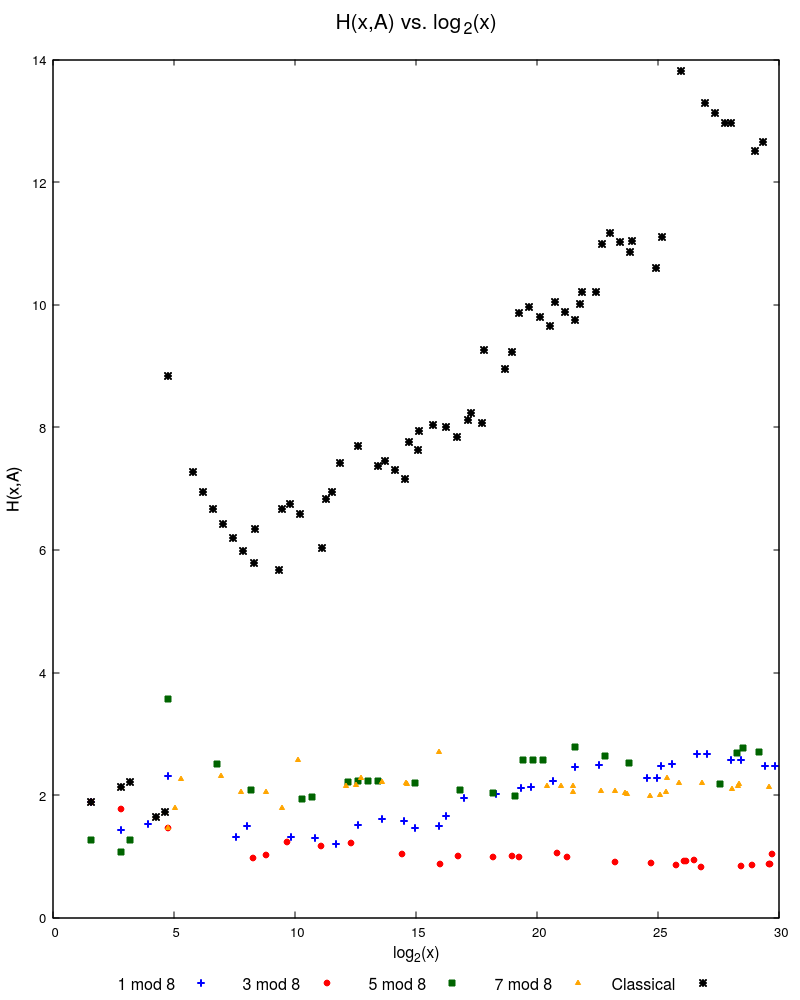
\includegraphics[scale=0.6]{ModAvoidanceAnalysisPics/H_vs_log.png}
    \caption{This graph visualizes how, for records $r$, the $H$ values for Collatz Variants 1, 3, 5, and 7 compare to each other, and how they compare to $H_C$. The number of bits for the records ($\log_2{N}$) is the x-axis, and the hardness measure $H$ as defined in Subsection~\ref{subsec:algdefinemeasure} is the y-axis.}
    \label{fig:hvslog}
\end{figure}

Comparing the unknown variants to themselves, there is no consistent leader among the three as the number of bits increases. However, they all seem to be within a hardness range of 1-3, with only a couple of exceptions. Variant 7 seems to remain in the same range with no definite increase or decrease, whereas variants 1 and 5 grow slightly from about 12 bits onward. The growth for both variants 1 and 5 may be because as numbers get larger, there are more opportunities to visit the $6 \rightarrow 7 \rightarrow 6$ cycle, which adds odd numbers more quickly to the sequence than any other base 8 graph traversal. More experiments for higher numbers should be consider in order to determine whether any of these three unknown variants continue to trend the same way.\par
Classical hardness actually tends to grow linearly against the log scale, meaning that as the input number increases in number of bits, $H_C$ increases logarithmically. This contrasts to $H$ for all the plotted Collatz Variants, which tend to stay below an $H$ of 3, meaning that figuring out proofs for the variants' termination is expected to be easier than proving the Collatz Conjecture.
\subsection{Percentage of Sequence Function Results and Analysis} \label{subsubsec:algsinpercentage}
 Figure~\ref{fig:pvslog} shows, for records $r$, the results of $P(r,A)$ versus the number of bitsin $r$. $P(N,A)$, as discussed earlier, is just calculating what percentage of odd numbers are part of record sequences for Collatz Variants 1, 3, 5, and 7. \par
\begin{figure}
    \centering
    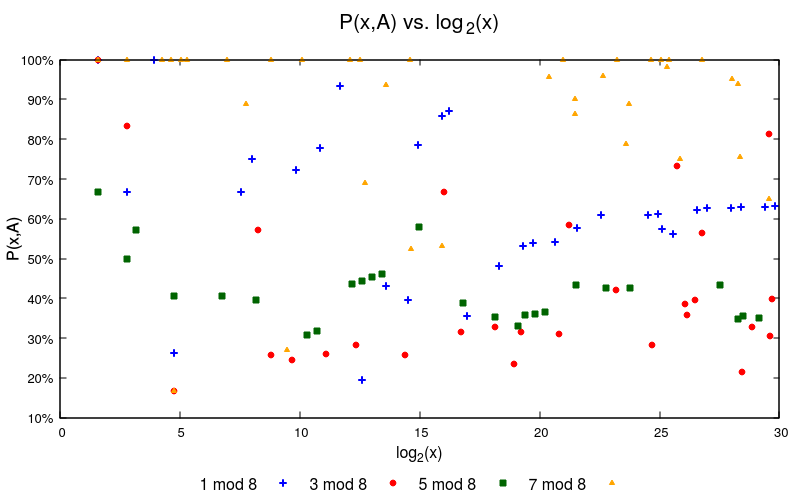
\includegraphics[scale=0.6]{ModAvoidanceAnalysisPics/P_vs_log.png}
    \caption{This graph visualizes how, for records $r$, $P$ values for Collatz Variants 1, 3, 5, and 7 compare to each other. The number of bits for the records ($\log_2{N}$) is the x-axis, and the percentage measure $P$ as defined in Subsection~\ref{subsec:algdefinemeasure} is the y-axis.}
    \label{fig:pvslog}
\end{figure}
Collatz Variant 7 comprises the highest percentage overall, with a couple of exceptions. Following Collatz Variant 7 causes the sequence to decline rapidly, since the $6 \rightarrow 7 \rightarrow 6$ cycle causes an input number to grow faster than any other cycle in the base 8 graph. Almost all of the records for variant 7 terminate at 1 instead of actually reaching a number that is $7 \Mod{8}$. \par
Variant 5 tends to have a low percentage, and appears to be the least erratic of all four variants. Variant 5 avoids the 0 self-cycle, which causes many divisions by 2. Numbers having record sequences that avoid $5 \Mod{8}$ tend to turn into very large numbers when variant 5 terminates, meaning that many more steps in the $3N+1$ mapping must often be taken before these numbers converge to 1. \par
Variant 1 is interesting, because as the input numbers grow larger, the line changes from erratic behavior to a more steady percentage at around 20 bits. This is likely a consequence of the sequence similarity that is seen in larger records for variant 1, which will be analyzed in Subsection~\ref{subsubsec:algseqsim}. Further, as mentioned in the cycle analysis in Subsection~\ref{subsubsec:cycleanalysis}, the $4 \rightarrow 6 \rightarrow 3 \rightarrow 2 \rightarrow 5 \rightarrow 0 \rightarrow \ldots \rightarrow 4$ cycle combined with the  $6 \rightarrow 7 \rightarrow 6$ cycle causes a clash between the decay of the 0 self-cycle and the growth of the $6 \rightarrow 7 \rightarrow 6$ cycle. This may explain some of the erratic percentage for variant 1, aside from the small part with chain similarity. \par
Variant 3 record sequences tend to have the lowest percentage of all odd numbers compared to other variants, even lower than variant 5, but also has erratic percentage. This could be explained by the fact that avoiding termination of variant 3 causes the sequence to follow some combination of the $6 \rightarrow 7 \rightarrow 6$ cycle, the $4 \rightarrow 2 \rightarrow 1 \rightarrow 4$ cycle, or the $4 \rightarrow 2 \rightarrow 5 \rightarrow 0  \rightarrow \ldots \rightarrow 4$ cycle with some number of $0$ self-cycles. The first cycle causes growth, whereas both other cycles cause decay. If the growth cycle is followed, the number gets larger, likely reducing the percentage of odd numbers making up long chains avoiding termination of variant 3, whereas the decay cycles cause the number to shrink, tending the percentages to be higher. This may explain why variant 3 causes widely different percentages.
\subsection{Sequence Similarity Analysis} \label{subsubsec:algseqsim}
We analyzed the sequences of the records for Collatz Variants 1, 5, and 7 as well to see if we could find any similarities:
\begin{itemize}
    \item Variant 1: There are two groups of records that were particularly interesting: Those from 325,791 to 32,505,681 (call this group $S$), and those from 35,651,835 to 949,643,331 (call this group $T$). Group $S$ numbers all terminated at number 161, and group $T$ numbers all terminated at number 35,369. These sequences all matched \textit{number-by-number} at least one other sequence starting at most 8 steps from the beginning. This is a striking similarity meaning that records for variant 1 might be predictably related to groups $S$ or $T$, or perhaps to other groups.
    \item Variant 7: All record sequences, except for input number 27, terminated at 1. While there was some similarity between sequences (all numbers $\geq 62079$ had the same last 41 numbers), there were many different paths taken from the input, so not as many patterns as variant 1.
    \item Variant 5: This had few matches and was the most changing of the records, so chain similarity appears not to have affected the low variance that $P$ has for variant 5.
\end{itemize}
\section{Paired Base Avoidance Analysis} \label{subsec:algpairedbase}
Since termination of Collatz Variants 1, 5, and 7 appear to be difficult to prove, we also analyzed two element combinations of them. The termination of two such variants were already proved in Subsection~\ref{subsubsec:base8subprob}: $\{1,5\}$ and $\{1,7\}$. However, termination of variant $\{5,7\}$ has yet to be proven. This section will analyze what happens to $H(N,A)$ and $P(N,A)$ where $A=\{1,5\}$, $\{1,7\}$, and $\{5,7\}$.
\subsection{Hardness Function Results and Analysis} \label{subsubsec:algmulhardness}
\begin{figure}
    \centering
    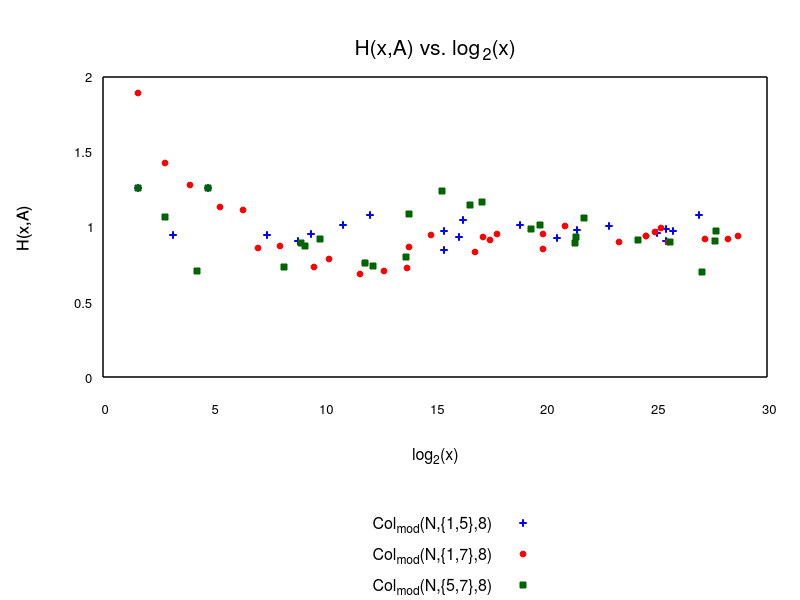
\includegraphics[scale=0.6]{ModAvoidanceAnalysisPics/H_vs_log_multi_base.png}
    \caption{This graph visualizes how, for records $r$, $H$ measure for the three Collatz Variants $\{1,5\}$, $\{1,7\}$, and $\{5,7\}$. The number of bits for the records ($\log_2{N}$) is the x-axis, and the hardness measure $H$ as defined in Subsection~\ref{subsec:algdefinemeasure} is the y-axis. Classical hardness was omitted from this graph to eliminate distortion.}
    \label{fig:h_multivslog}
\end{figure}
Figure~\ref{fig:h_multivslog} shows, for records $r$, $H(r,A)$ versus bits in $r$. These results were quite surprising. At first thought, it would have appeared that the unproven variant $\{5, 7\}$ should be the hardest to determine, compared to the two variants we have proofs for. But both variants $\{1, 5\}$ and $\{1, 7\}$  had alike predictive hardness to $\{5, 7\}$! These numbers suggest that a proof for determining why variant $\{5, 7\}$ must terminate is either easier than we anticipated, or our hardness measures are not very good. However, given the fact that variant 3 for the single base cases is clearly easier than variants 1, 5, and 7, we have reason to believe this measure should be good. Further investigation needs to be considered.
\subsection{Percentage of Sequence Function Results and Analysis} \label{subsubsec:algmulpercentage}
\begin{figure}
    \centering
    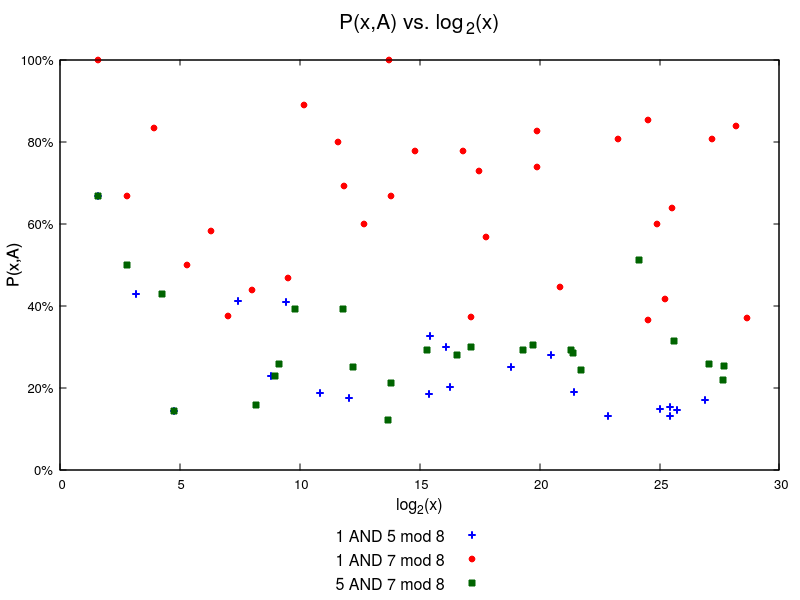
\includegraphics[scale=0.6]{ModAvoidanceAnalysisPics/P_vs_log_multi_base.png}
    \caption{This graph visualizes how, for records $r$, the $P$ measure for variants $\{1,5\}$, $\{1,7\}$, and $\{5,7\}$. The number of bits for the records ($\log_2{N}$) is the x-axis, and the hardness measure $P$ as defined in Subsection~\ref{subsec:algdefinemeasure} is the y-axis.}
    \label{fig:p_multi_vslog}
\end{figure}
Figure~\ref{fig:p_multi_vslog} shows, for records $r$, $P(r,A)$ versus bits in $r$. Record sequences for variant $\{1,7\}$ make up the highest percentage of their overall Collatz Sequences, because avoiding both the $6 \rightarrow 7 \rightarrow 6$ and the $4 \rightarrow 6 \rightarrow 3 \rightarrow 2 \rightarrow 1 \rightarrow 4$ cycles allows for the sequence to only go through the $4  \rightarrow 2 \rightarrow 5 \rightarrow 0 \rightarrow \ldots \rightarrow 4$ cycle, causing fast decay, like variant 7. \par
Both variants $\{1,5\}$ and $\{5,7\}$ are much closer to each other in the percentage that their Record Collatz Variant Sequences comprise of their $3N+1$ sequences, although as the numbers grow past 17 bits in size, variant $\{5,7\}$ comprises of the higher percentage. A possible explanation is the fact that the $6 \rightarrow 7 \rightarrow 6$ cycle allowed in variant $\{1,5\}$, but not variant $\{5,7\}$, causes a number to grow larger than the $4 \rightarrow 6 \rightarrow 3 \rightarrow 2 \rightarrow 1$ cycle that variant $\{5,7\}$ allows. \hl{Also, since variant $\{1,5\}$ allows for larger numbers, and larger numbers generally (but not always) take more steps to decline, allowing for more growth should mean that Record Collatz Variant $\{1,5\}$ Sequences comprise a lower percentage of all odd numbers in record numbers' overall $3N+1$ sequences.}

%%  LocalWords:  Lagrias Roosendaal baseavoid csv entirechain updown
%%  LocalWords:  untildecay README avoidingmodgrowth GBs GitHub
%%  LocalWords:  readme logarithmically
